% =====================================================================
\chapter{Le processus d'Ornstein-Uhlenbeck}
\label{ch:5}
% =====================================================================

\section{Objectifs et organisation du chapitre}

\paragraph{Objectifs.} Le processus d'Ornstein-Uhlenbeck (OU) est la version en temps continu de l'AR(1). Il est devenu le modèle standard de l'écart en arbitrage statistique \citep{avellaneda2010,bertram2010,leungli2016}, parce qu'il permet de calculer explicitement des durées de détention et des seuils optimaux. À la fin du chapitre, vous saurez : (1) ce qu'est un mouvement brownien et une équation différentielle stochastique ; (2) appliquer le lemme d'Itô pour résoudre l'équation d'OU ; (3) passer exactement de l'OU à l'AR(1) et inversement, et estimer les paramètres ; (4) calculer le temps moyen de retour à la moyenne par l'équation de Kolmogorov ; (5) choisir des seuils d'entrée qui maximisent le gain par unité de temps en présence de coûts.

\paragraph{Code.} \texttt{code/ch05/ch05\_ornstein\_uhlenbeck.py}, expériences E1 à E5.

% =====================================================================
\section{Mouvement brownien et équations différentielles stochastiques}
% =====================================================================

\subsection{Le mouvement brownien}

\begin{definition}
Un mouvement brownien standard $(W_t)_{t\ge0}$ est un processus en temps continu tel que $W_0 = 0$, ses trajectoires sont continues, et pour $s<t$ l'accroissement $W_t - W_s$ suit une loi $\N(0, t-s)$, indépendante de tout ce qui s'est passé avant $s$.
\end{definition}

C'est la limite de la marche aléatoire du chapitre~1 quand on fait des pas de plus en plus petits et de plus en plus fréquents. Sur un petit intervalle $\dd t$, l'accroissement $\dd W_t$ est d'ordre $\sqrt{\dd t}$ (son écart-type), et non $\dd t$. Conséquence capitale : $(\dd W_t)^2$, d'espérance $\dd t$ et de variance $2\dd t^2$, se comporte comme la quantité déterministe $\dd t$ ; on écrit $(\dd W_t)^2 = \dd t$.

\subsection{Équation différentielle stochastique}

Une équation différentielle stochastique (EDS) décrit l'évolution infinitésimale d'un processus :
\[
\dd X_t = b(X_t)\,\dd t + s(X_t)\,\dd W_t,
\]
où $b$ est la \emph{dérive} (la tendance locale) et $s$ la \emph{volatilité}. On la lit comme la limite de $X_{t+\Delta} - X_t \approx b(X_t)\Delta + s(X_t)\sqrt\Delta\,Z$, avec $Z\sim\N(0,1)$.

\subsection{Le lemme d'Itô}

\begin{proposition}[Lemme d'Itô, forme simple]
Si $\dd X_t = b\,\dd t + s\,\dd W_t$ et si $f(t,x)$ est deux fois dérivable, alors
\[
\dd f(t, X_t) = \Big(\partial_t f + b\,\partial_x f + \tfrac12 s^2\,\partial_{xx}f\Big)\dd t + s\,\partial_x f\,\dd W_t.
\]
\end{proposition}
\begin{proof}[Idée de la démonstration]
On développe $f$ à l'ordre 2 : $\dd f = \partial_t f\,\dd t + \partial_x f\,\dd X + \frac12\partial_{xx}f\,(\dd X)^2 + \dots$ Or $(\dd X)^2 = b^2\dd t^2 + 2bs\,\dd t\,\dd W + s^2(\dd W)^2$ ; les deux premiers termes sont négligeables (d'ordre $\dd t^{3/2}$ ou plus) et le troisième vaut $s^2\dd t$. On remplace $\dd X$ par $b\,\dd t + s\,\dd W$ et on regroupe.
\end{proof}

Le terme $\frac12 s^2\partial_{xx}f$ n'existe pas en calcul ordinaire : il vient de ce que le hasard brownien a une variance d'ordre $\dd t$.

% =====================================================================
\section{Le processus d'Ornstein-Uhlenbeck}
% =====================================================================

\subsection{Définition et solution}

\begin{definition}[\citet{uhlenbeck1930}]
Le processus d'Ornstein-Uhlenbeck est la solution de
\[
\dd X_t = \theta(\mu - X_t)\,\dd t + \sigma\,\dd W_t, \qquad \theta>0,\ \sigma>0.
\]
\end{definition}

La dérive $\theta(\mu - X_t)$ tire le processus vers $\mu$ avec une force proportionnelle à l'écart : c'est l'élastique du chapitre~1, en temps continu. $\theta$ est la \emph{vitesse de retour}, $\mu$ le niveau d'équilibre, $\sigma$ la volatilité instantanée.

\begin{proposition}\label{c5:prop:sol}
La solution vaut
\[
X_t = \mu + (X_0-\mu)e^{-\theta t} + \sigma\int_0^t e^{-\theta(t-u)}\,\dd W_u,
\]
de sorte que, sachant $X_0$, $X_t$ suit une loi normale de moyenne $\mu + (X_0-\mu)e^{-\theta t}$ et de variance $\frac{\sigma^2}{2\theta}\big(1-e^{-2\theta t}\big)$.
\end{proposition}
\begin{proof}
On applique le lemme d'Itô à $f(t,x) = e^{\theta t}x$ : $\partial_t f = \theta e^{\theta t}x$, $\partial_x f = e^{\theta t}$, $\partial_{xx}f = 0$. Donc
\[
\dd(e^{\theta t}X_t) = \big(\theta e^{\theta t}X_t + \theta(\mu - X_t)e^{\theta t}\big)\dd t + \sigma e^{\theta t}\dd W_t = \theta\mu\,e^{\theta t}\dd t + \sigma e^{\theta t}\dd W_t.
\]
Les termes en $X_t$ se sont annulés. On intègre de 0 à $t$ : $e^{\theta t}X_t - X_0 = \mu(e^{\theta t} - 1) + \sigma\int_0^t e^{\theta u}\dd W_u$, puis on multiplie par $e^{-\theta t}$. L'intégrale stochastique a une espérance nulle ; sa variance vaut, par la propriété d'isométrie (la variance d'une intégrale brownienne est l'intégrale du carré de l'intégrande), $\sigma^2\int_0^t e^{-2\theta(t-u)}\dd u = \frac{\sigma^2}{2\theta}(1-e^{-2\theta t})$.
\end{proof}

\paragraph{Conséquences.} Quand $t\to\infty$, la loi de $X_t$ tend vers la loi stationnaire $\N\big(\mu, \sigma^2/(2\theta)\big)$. L'écart-type stationnaire $\sigma_{eq} = \sigma/\sqrt{2\theta}$ est l'unité naturelle pour placer les seuils de trading. L'écart espéré à la moyenne est divisé par deux en
\[
h_{1/2} = \frac{\ln 2}{\theta}.
\]

\begin{figure}[h]
\centering
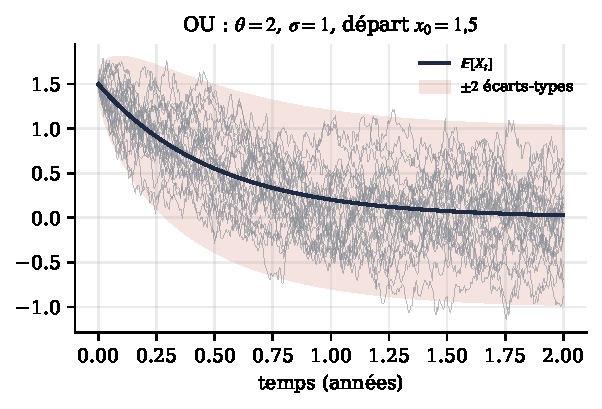
\includegraphics[width=0.62\textwidth]{ch05/ou_trajectoires.pdf}
\caption{Trajectoires d'un OU partant de $x_0 = 1{,}5$ : la moyenne décroît exponentiellement vers 0 et la dispersion converge vers $\pm2\sigma_{eq}$.}
\label{c5:fig:paths}
\end{figure}

\subsection{De l'OU à l'AR(1), exactement}

En observant le processus à intervalles réguliers $\Delta$ (un jour, $\Delta = 1/252$ an), la proposition~\ref{c5:prop:sol} appliquée entre $t$ et $t+\Delta$ donne exactement
\[
X_{t+\Delta} = \mu + e^{-\theta\Delta}(X_t - \mu) + \eta_t, \qquad \eta_t \sim \N\Big(0,\ \frac{\sigma^2}{2\theta}\big(1-e^{-2\theta\Delta}\big)\Big),
\]
c'est-à-dire un AR(1) avec
\[
\varphi = e^{-\theta\Delta}, \qquad \sigma_\eta^2 = \frac{\sigma^2}{2\theta}(1-\varphi^2).
\]
Inversement, une estimation $\hat\varphi$ de l'AR(1) donne $\hat\theta = -\ln\hat\varphi/\Delta$ et $\hat\sigma = \hat\sigma_\eta\sqrt{2\hat\theta/(1-\hat\varphi^2)}$. Le schéma d'Euler, $X_{t+\Delta} = X_t + \theta(\mu - X_t)\Delta + \sigma\sqrt\Delta Z$, n'est qu'une approximation : il remplace $e^{-\theta\Delta}$ par $1-\theta\Delta$.

\begin{codebox}[ — E1, discrétisation exacte contre Euler]
\textbf{Protocole :} $\theta = 2$ (demi-vie de $0{,}35$ an), $\sigma = 1$, variance stationnaire théorique $0{,}25$. \textbf{Résultats :} pas quotidien ($\Delta = 1/252$) : les deux schémas donnent une autocorrélation de $0{,}992$, identique à la théorie. Pas mensuel : exact $0{,}846$ (théorie $0{,}847$), Euler $0{,}830$ ; variance Euler $0{,}273$. Pas trimestriel : exact $0{,}610$ (théorie $0{,}607$), Euler $0{,}505$ ; variance Euler $0{,}324$, soit 30\,\% de trop. \textbf{Leçon :} simulez toujours avec la discrétisation exacte, qui est aussi simple à coder.
\end{codebox}

\subsection{Estimation}

\begin{codebox}[ — E2, estimation des paramètres]
\textbf{Protocole :} $\theta = 5$ (demi-vie de 35 jours), $\mu = 1$, $\sigma = 0{,}5$ ; 500 trajectoires quotidiennes par durée. \textbf{Résultats} (médiane et intervalle 5–95\,\% de $\hat\theta$) : 1 an : $8{,}65$ $[2{,}8\,;\,20{,}6]$ ; 4 ans : $5{,}81$ $[3{,}4\,;\,9{,}8]$ ; 16 ans : $5{,}22$ $[4{,}0\,;\,6{,}8]$. $\hat\sigma$ est très précis dès un an (médiane $0{,}504$), $\hat\mu$ l'est beaucoup moins (écart-type $0{,}12$ sur un an pour un écart-type stationnaire de $0{,}16$).
\end{codebox}

\begin{pitfall}
Sur un an, la vitesse de retour est surestimée de 70\,\% en médiane, ce qui divise la demi-vie apparente presque par deux : c'est le biais de Kendall du chapitre~2, traduit en temps continu. La moyenne $\mu$ est elle aussi mal connue, alors que tous les seuils de trading sont placés autour d'elle. La volatilité, elle, est bien estimée : c'est le paramètre le plus fiable et le moins important pour la décision.
\end{pitfall}

% =====================================================================
\section{Combien de temps pour revenir ? Les temps de premier passage}
% =====================================================================

\subsection{L'équation de Kolmogorov}

Notons $u(x)$ le temps moyen que met le processus, parti de $x$, pour atteindre un niveau cible. Pendant un court instant $\dd t$, il s'écoule $\dd t$ et le processus passe de $x$ à $x + \dd X$ ; ensuite, il reste en moyenne $u(x+\dd X)$ :
\[
u(x) = \dd t + \E\big[u(x + \dd X)\big].
\]
On développe $u$ à l'ordre 2 et l'on utilise $\E[\dd X] = b(x)\dd t$ et $\E[(\dd X)^2] = s(x)^2\dd t$ :
\[
u(x) = \dd t + u(x) + b(x)u'(x)\dd t + \tfrac12 s(x)^2u''(x)\dd t \quad\Longrightarrow\quad \tfrac12 s(x)^2u''(x) + b(x)u'(x) = -1.
\]
C'est l'équation de Kolmogorov rétrograde pour les temps moyens de sortie.

\subsection{Résolution pour l'OU}

Prenons $\mu = 0$ (on mesure l'écart à la moyenne), $b(x) = -\theta x$, $s = \sigma$, et posons $k = \theta/\sigma^2$, $v = u'$. L'équation devient $\frac{\sigma^2}{2}v' - \theta x\,v = -1$. En multipliant par le facteur intégrant $\frac{2}{\sigma^2}e^{-kx^2}$, le membre de gauche devient une dérivée exacte :
\[
\frac{\dd}{\dd x}\Big(v(x)\,e^{-kx^2}\Big) = -\frac{2}{\sigma^2}e^{-kx^2}.
\]

\begin{proposition}[Temps moyens de passage de l'OU]\label{c5:prop:fpt}
Avec $k = \theta/\sigma^2$ et un seuil $a>0$ :
\begin{align*}
\text{(retour)}\quad T_{a\to 0} &= \frac{2}{\sigma^2}\int_0^a e^{ky^2}\Big(\int_y^{\infty}e^{-kz^2}\dd z\Big)\dd y,\\
\text{(attente)}\quad T_{0\to\pm a} &= \frac{2}{\sigma^2}\int_0^a e^{ky^2}\Big(\int_0^{y}e^{-kz^2}\dd z\Big)\dd y,
\end{align*}
où $T_{a\to0}$ est le temps moyen pour revenir de $a$ à la moyenne, et $T_{0\to\pm a}$ celui pour s'écarter de la moyenne jusqu'à $|x| = a$.
\end{proposition}
\begin{proof}
\emph{Retour.} La cible est 0 et le processus part de $x>0$ ; loin vers le haut, la force de rappel est énorme, ce qui impose $v(x)e^{-kx^2}\to0$ quand $x\to\infty$. On intègre l'équation entre $y$ et $+\infty$ : $0 - v(y)e^{-ky^2} = -\frac{2}{\sigma^2}\int_y^\infty e^{-kz^2}\dd z$, d'où $v(y)$. Comme $u(0) = 0$ (on est déjà arrivé), $u(a) = \int_0^a v(y)\,\dd y$.

\emph{Attente.} Les cibles sont $\pm a$ et le départ est 0 ; par symétrie $u'(0) = 0$. On intègre entre 0 et $y$ : $v(y)e^{-ky^2} = -\frac{2}{\sigma^2}\int_0^ye^{-kz^2}\dd z$. Comme $u(a) = 0$, $u(0) = u(a) - \int_0^a v(y)\dd y$, ce qui donne la formule.
\end{proof}

Les intégrales intérieures s'écrivent avec la fonction d'erreur ($\int_0^ye^{-kz^2}\dd z = \frac12\sqrt{\pi/k}\,\mathrm{erf}(\sqrt k\,y)$), et l'intégrale extérieure se calcule numériquement.

\begin{codebox}[ — E3, temps de passage : formule contre simulation]
\textbf{Protocole :} $\theta = \sigma = 1$, 4\,000 trajectoires au pas $10^{-3}$ par seuil. \textbf{Résultats} (seuils en écarts-types stationnaires) :
\begin{center}\small
\begin{tabular}{lcccc}
\toprule
$a/\sigma_{eq}$ & $T_{a\to0}$ formule & simulé & $T_{0\to\pm a}$ formule & simulé\\
\midrule
0,5 & 0,523 & 0,546 & 0,130 & 0,146\\
1,0 & 0,902 & 0,951 & 0,596 & 0,637\\
1,5 & 1,192 & 1,233 & 1,711 & 1,789\\
2,0 & 1,425 & 1,468 & 4,502 & 4,726\\
\bottomrule
\end{tabular}
\end{center}
Les temps simulés sont 3 à 10\,\% plus longs : en temps discret, on ne voit le franchissement qu'au pas suivant (biais de surveillance discrète, d'ordre $\sqrt{\Delta}$).
\end{codebox}

\paragraph{Lecture.} Revenir d'un écart de $2\sigma_{eq}$ prend environ $1{,}4/\theta$, soit deux demi-vies ; mais \emph{attendre} un écart de $2\sigma_{eq}$ prend $4{,}5/\theta$, trois fois plus. Les seuils larges font de bons trades, mais rares.

% =====================================================================
\section{Seuils de trading optimaux}
% =====================================================================

\subsection{Le problème}

Considérons la stratégie symétrique : on attend que l'écart atteigne $\pm a$, on prend la position opposée, et on la ferme quand l'écart revient à la moyenne. Chaque cycle rapporte $a$ (en unités d'écart) moins un coût $c$ par aller-retour, et dure en moyenne $T_{0\to\pm a} + T_{a\to0}$. Par la loi des grands nombres, le gain moyen par unité de temps est
\[
G(a) = \frac{a - c}{T_{0\to\pm a}(a) + T_{a\to0}(a)}.
\]
\citet{bertram2010} étudie ce critère et sa version ajustée du risque ; \citet{leungli2015} traitent le problème comme un double arrêt optimal (quand entrer, puis quand sortir) avec coûts et stop-loss.

\begin{intuition}
Un seuil bas fait beaucoup de petits trades ; un seuil haut fait peu de gros trades. Sans coûts, rien n'empêche de trader de minuscules écarts en continu. Avec des coûts, chaque trade doit d'abord rembourser son ticket d'entrée : le seuil optimal monte avec les coûts.
\end{intuition}

\begin{codebox}[ — E4, seuil optimal]
\textbf{Résultats} ($\theta = \sigma = 1$, seuils et coûts en écarts-types stationnaires) : sans coût, le gain par unité de temps est maximal pour un seuil qui tend vers 0, artefact du temps continu. Avec un coût de $0{,}1$ : seuil optimal $0{,}69$ ; coût $0{,}25$ : $0{,}97$ ; coût $0{,}5$ : $1{,}26$ (figure~\ref{c5:fig:opt}). \textbf{Vérification en temps quotidien} (demi-vie de 14 jours, 400 ans simulés) : avec un coût de $0{,}25$, gain annuel simulé de $6{,}5$ et $5{,}0$ écarts-types pour $a = 1$ et $1{,}5$, contre $6{,}3$ et $5{,}4$ par la formule. Pour les petits seuils, la simulation gagne nettement plus que la formule ($5{,}9$ contre 0 pour $a = c = 0{,}25$) : en temps discret, la clôture dépasse souvent le seuil, ce qui \og offre\fg{} un meilleur prix d'entrée et de sortie.
\end{codebox}

\begin{figure}[h]
\centering
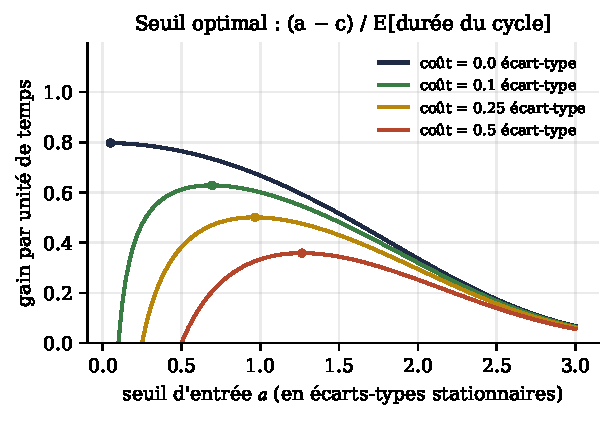
\includegraphics[width=0.62\textwidth]{ch05/seuils_optimaux.pdf}
\caption{Gain par unité de temps en fonction du seuil d'entrée pour quatre niveaux de coût. Le point marque l'optimum.}
\label{c5:fig:opt}
\end{figure}

\begin{pitfall}
Le gain \og offert\fg{} par le dépassement en temps discret est une illusion de \emph{backtest} si, dans la réalité, on exécute par ordres limites au seuil (on n'obtient jamais mieux que le seuil, et l'on n'est exécuté que quand le prix traverse, souvent au pire moment : chapitre~15) ou si l'on exécute au marché le lendemain (on paie le retour partiel). Un \emph{backtest} de \emph{pairs trading} au prix de clôture surestime systématiquement les stratégies à seuils serrés.
\end{pitfall}

\subsection{Seuils et incertitude sur les paramètres}

Le seuil optimal dépend de $\theta$, $\mu$ et $\sigma$. Or E2 a montré que $\theta$ est surestimé et que $\mu$ est mal connu sur un an. Un seuil optimisé sur des paramètres estimés est donc lui-même incertain, et généralement trop serré (car $\theta$ surestimé fait croire que les cycles sont plus courts). En pratique : corriger le biais de $\hat\theta$, élargir légèrement les seuils et vérifier la robustesse sur une plage de paramètres plutôt qu'en un point.

% =====================================================================
\section{Étude de cas : l'écart GLD/GLDM}
% =====================================================================

Sur l'écart GLD/GLDM sans tendance (chapitre~3), $\hat\varphi = 0{,}011$ à l'échelle quotidienne : un OU avec $\theta\Delta = -\ln 0{,}011 \approx 4{,}5$, c'est-à-dire une demi-vie d'environ $0{,}15$ jour, soit une heure de bourse. À l'échelle quotidienne, l'écart (écart-type $4{,}5$ pb) est indiscernable d'un bruit blanc. La modélisation OU n'a d'intérêt que si l'on observe le processus à une fréquence comparable à sa demi-vie : pour cet écart, des données intrajournalières seraient indispensables.

% =====================================================================
\section{Ce que la théorie apporte, et ses limites}
% =====================================================================

\paragraph{Apports.} Un modèle à trois paramètres interprétables ($\theta$, $\mu$, $\sigma$), une correspondance exacte avec l'AR(1) à toute fréquence, des formules de durée de détention et un critère explicite pour choisir les seuils en fonction des coûts.

\paragraph{Limites.} (1) Les chocs browniens sont gaussiens ; les écarts réels ont des queues épaisses et des sauts (annonces de résultats, dividendes). (2) Les paramètres sont supposés constants. (3) Le critère \og gain par unité de temps\fg{} ignore le risque : un seuil qui maximise l'espérance peut avoir une variance déplaisante ; il ignore aussi le capital immobilisé et la marge. (4) La surveillance discrète, l'exécution et les coûts réels changent les résultats, surtout pour les seuils serrés.

% =====================================================================
\section{Fiche à recopier au tableau blanc}
% =====================================================================

\begin{whiteboard}
\begin{itemize}[leftmargin=1.2em]
\item \textbf{Brownien :} $W_t - W_s\sim\N(0,t-s)$, $(\dd W)^2 = \dd t$.
\item \textbf{Itô :} $\dd f = (\partial_tf + b\,\partial_xf + \frac12s^2\partial_{xx}f)\dd t + s\,\partial_xf\,\dd W$.
\item \textbf{OU :} $\dd X = \theta(\mu - X)\dd t + \sigma\dd W$ ; $X_t = \mu + (X_0-\mu)e^{-\theta t} + \sigma\int_0^te^{-\theta(t-u)}\dd W_u$.
\item \textbf{Moments :} moyenne $\mu + (X_0-\mu)e^{-\theta t}$ ; variance $\frac{\sigma^2}{2\theta}(1-e^{-2\theta t})$ ; $\sigma_{eq} = \sigma/\sqrt{2\theta}$ ; $h_{1/2} = \ln2/\theta$.
\item \textbf{OU $\leftrightarrow$ AR(1) :} $\varphi = e^{-\theta\Delta}$, $\sigma_\eta^2 = \frac{\sigma^2}{2\theta}(1-\varphi^2)$ ; $\hat\theta = -\ln\hat\varphi/\Delta$.
\item \textbf{Kolmogorov :} $\frac12s^2u'' + bu' = -1$.
\item \textbf{Retour :} $T_{a\to0} = \frac2{\sigma^2}\int_0^ae^{ky^2}\int_y^\infty e^{-kz^2}\dd z\,\dd y$, $k=\theta/\sigma^2$.
\item \textbf{Seuil optimal :} maximiser $(a-c)/(T_{0\to\pm a}+T_{a\to0})$ ; le seuil monte avec les coûts.
\end{itemize}
\end{whiteboard}

% =====================================================================
\section{Exercices}
% =====================================================================

\begin{exercise}
Appliquez le lemme d'Itô à $f(x) = x^2$ pour un mouvement brownien $X = W$. Déduisez-en $\E[W_t^2] = t$.
\end{exercise}

\begin{exercise}
Un écart quotidien a $\hat\varphi = 0{,}96$ et un écart-type des résidus de 0,5\,\%. Calculez $\theta$ (par an), la demi-vie en jours et l'écart-type stationnaire.
\end{exercise}

\begin{exercise}
Montrez, en dérivant l'intégrale de la proposition~\ref{c5:prop:fpt}, que pour un petit seuil $a$, $T_{a\to0}\approx a\sqrt{\pi/\theta}/\sigma$. Pourquoi ce temps tend-il vers 0 avec $a$ alors que celui d'un mouvement brownien sans dérive serait infini en moyenne ?
\end{exercise}

\begin{exercise}[à coder]
Ajoutez à E4 un stop-loss : on ferme à perte si l'écart atteint $\pm L$ avec $L > a$. Comment le seuil optimal et le gain changent-ils pour $L = 3\sigma_{eq}$ ? Comparez à \citet{leungli2015}.
\end{exercise}

\begin{exercise}[à coder]
Reprenez E2 avec la correction de Kendall appliquée à $\hat\varphi$ avant de calculer $\hat\theta$. Quel est le nouveau biais médian sur un an ?
\end{exercise}

% =====================================================================
\section{Pour aller plus loin}
% =====================================================================

\begin{toread}
\begin{itemize}[leftmargin=1.2em]
\item \citet{uhlenbeck1930} : l'article original, en physique.
\item \citet{bertram2010} : expressions analytiques du gain et de la durée des cycles, et seuils optimaux.
\item \citet{leungli2015} et les premiers chapitres du livre \citet{leungli2016} : entrée et sortie optimales avec coûts et stop-loss.
\item \citet{avellaneda2010}, l'annexe sur l'estimation des paramètres OU à partir d'une régression AR(1), reprise au chapitre~10.
\end{itemize}
\end{toread}

\section{Scripts du chapitre}
\noindent\texttt{code/ch05/ch05\_ornstein\_uhlenbeck.py} : E1 (figure~\ref{c5:fig:paths}), E2, E3, E4 (figure~\ref{c5:fig:opt}), E5.
